% +--------------------------------------------------------------------+
% | LaTeX Template                                                     |
% | for K-State Electronic Theses, Dissertations, and Reports          |
% |                                                                    |
% | Comments and guidelines for using the template are shown           |
% | within boxes like this one.                                        |
% |                                                                    |
% | Revised 6/30/06                                                    |
% | 9/14/06: Removed typos                                             |
% +--------------------------------------------------------------------+

% +--------------------------------------------------------------------+
% | Your paper should contain the following sections, except where     |
% | indicated as optional, in the order shown.  Also, all headings     |
% | shown with an asterisk (*) must be centered and in uppercase       |
% | letters:                                                           |
% |                                                                    |
% | Abstract Title Page (doctoral dissertations only)                  |
% | ABSTRACT* (doctoral dissertations only)                            |
% | Title Page                                                         |
% | Copyright Page (Optional - only needed if copyrighting)            |
% | ABSTRACT *                                                         |
% | TABLE OF CONTENTS *                                                |
% | LIST OF FIGURES *                                                  |
% | LIST OF TABLES*                                                    |
% | ACKNOWLEDGMENTS* (Optional)                                        |
% | DEDICATION * (Optional)                                            |
% | PREFACE * (Optional)                                               |
% | Individual Chapters                                                |
% | References and/or bibliography                                     |
% | Appendices (as needed)                                             |
% +--------------------------------------------------------------------+

% +--------------------------------------------------------------------+
% | The LaTex keyword \documentclass selects a particular class to     |
% | associate with the document.  The current documentclass            |
% | {class_diss} generates a Table of Contents that has leading dots   |
% | only on chapter subheadings.  If you prefer a Table of Contents    |
% | that has leading dots for all entries, replace {class_diss}        |
% | with {Mydiss} in the command below.                                |
% |                                                                    |
% +--------------------------------------------------------------------+

\documentclass[final, 12pt,oneside]{class_diss}



% +--------------------------------------------------------------------+
% | The following command sets the bibliography style to American
% | Institute of Physics (AIP).  Other styles are available in the
% | styles directory.  To use a different style, replace "aip" with
% | the filename of the style you want to use.
% +--------------------------------------------------------------------+

\bibliographystyle{styles/plain}



% TODO acronimos
\usepackage[acronym]{glossaries}
\usepackage[automake]{glossaries-extra}
%\usepackage[spanish]{cleveref}

\makeglossaries

\usepackage{geometry}


\usepackage{listings}
\usepackage{mdframed} 
\usepackage[T1]{fontenc}

\usepackage{verbatim} % NO ES MUY BONITO
\usepackage[ruled,vlined]{algorithm2e} % ALGORITMOS COMO EN CODIGO DE RICARDO PEÑA

\usepackage{tcolorbox}
\usepackage{fancyvrb}
\usepackage[table]{xcolor}

\usepackage{colortbl}
\usepackage{array}
\usepackage{makecell}


\usepackage{pgfplots} 
\usepgfplotslibrary{groupplots}
\pgfplotsset{compat=1.17} % TODO ?

\usepgfplotslibrary{fillbetween}
\usetikzlibrary{patterns}
\usepackage{subcaption} % subfigures
\usepackage{caption}

% TODO ERROR
%\usepackage[hidelinks]{hyperref}
% TODO ERROR
%\usepackage[capitalise]{cleveref}
% TODO ERROR
%\crefname{table}{tabla}{tablas}

\usepackage[utf8]{inputenc}
\usepackage[T1]{fontenc}
\usepackage[spanish]{babel}
% +--------------------------------------------------------------------+
% | Now, we add in all external packages that we will use throughout   |
% | the document.  You can add other packages as needed.
% +--------------------------------------------------------------------+

%\usepackage{     caption2} % Customize captions a bit more
\usepackage{      amsmath} % American Mathematics Society standards
%\usepackage{      wrapfig} % Wraps text around a figure or table
\usepackage{     graphicx} % Extended graphics package.
%\usepackage{     fancyhdr} % Efficiently handles headers and footers
%\usepackage{       braket} % Bra-Ket notation package
%\usepackage{     mathrsfs} % Specialized Math fonts (Hamiltonian, etc.)
%\usepackage{boxedminipage} % Boxed text can be produced
%\usepackage{     setspace} % Controls line spacing via \begin{space}

\usepackage{amsxtra}
\usepackage{amssymb}
\usepackage{amsthm}
\usepackage{latexsym}

% +--------------------------------------------------------------------+
% | The color package allows one to select colors for hyperlinking     |
% | (see below).                                                       |
% +--------------------------------------------------------------------+

% TODO DA ERROR CON TODAS LAS LIBRERIAS
%\usepackage[usenames]{color}

% +--------------------------------------------------------------------+
% | Colors defined for use with this template.                         |
% +--------------------------------------------------------------------+

\definecolor{  Pink}{rgb}{1.0, 0.5, 0.5}
\definecolor{Maroon}{rgb}{0.8, 0.0, 0.0}

% +--------------------------------------------------------------------+
% | In the commands below, we use the 'natbib' package, and specify    |
% | the 'sort&compress' option, which condenses                        |
% | citations from (1,2,3,5,9,10,11) to (1-3,5,9-11).  The 'bibpunct'  |
% | option selects various parameters for how the citation will be     |
% | displayed.  In this case, only the comma (separation between       |
% | citations) and the 's' (superscript) arguments are chosen.  The    |
% | other curly braces deal with how to 'wrap' the citation (using     |
% | parentheses, brackets, etc.) and are not needed for the chosen     |
% | style.                                                             |
% +--------------------------------------------------------------------+

\usepackage[sort&compress]{natbib}
\bibpunct{}{}{,}{s}{}{}
\usepackage{hypernat}

% +--------------------------------------------------------------------+
% | Lastly, the hyperref package allows one to hyperlink cross-        |
% | references and figures in a LaTeX document.                        |
% +--------------------------------------------------------------------+

\usepackage[pdftex, plainpages=false, pdfpagelabels]{hyperref}

\hypersetup{
    linktocpage=true,
    colorlinks=true,
    bookmarks=true,
    citecolor=blue,
    urlcolor=red,
    linkcolor=Maroon,
    citebordercolor={1 0 0},
    urlbordercolor={1 0 0},
    linkbordercolor={.7 .8 .8},
    breaklinks=true,
    pdfpagelabels=true,
    }

% +--------------------------------------------------------------------+
% | Page margins are set on 1 inch on all sides.                       |
% +--------------------------------------------------------------------+

\topmargin      = -0.56in
\textheight     =  8.60in
\textwidth      =  6.46in
\oddsidemargin  =  0.02in

% +--------------------------------------------------------------------+
% | The document finally begins here.                                  |
% +--------------------------------------------------------------------+

\begin{document}


  \setcounter{page}{-1}


% +--------------------------------------------------------------------+
% | Title Page -- Required for both Doctoral and Masters Students
% +--------------------------------------------------------------------+

\begin{titlepage}
	%make sure this page is centered
	\newgeometry{top=2.25cm, bottom=2.25cm, outer=2.5cm, inner=2.5cm, heightrounded, marginparwidth=2.5cm, marginparsep=0.3cm}
	\thispagestyle{empty}
	
	\begin{center}
		
		\vspace{1cm}
		
		\vspace{0.65cm}
		\rule{2in}{0.5pt}\\
		\vspace{0.85cm}
		
		{\Large Optimization of AI algorithms by applying high-performance computing techniques}\\
		
		\vspace{0.65cm}
		\rule{2in}{0.5pt}\\
		\vspace{0.85cm}
		
		{\Large Optimización de algoritmos de IA aplicando técnicas enfocadas al cómputo de alto rendimiento}\\
		
		\vspace{0.65cm}
		\rule{2in}{0.5pt}\\
		
		
		
		\vfill
		
\includegraphics[height=2.5in]{images/escudo_ucm.pdf}
		\vfill
		
		
		
		\textbf{TRABAJO DE FIN DE GRADO}\\
		\vspace{0.7cm}
		\textbf{DANIEL PIZARRO GALLEGO}
		
		\vspace{1cm}
		
		Director:\\
		\textbf{Alberto Núñez Covarrubias}\\
		
		\vspace{1.8cm}
		Facultad de Informática\\
		Universidad Complutense de Madrid
		\vspace{0.5cm}
		
		XX de septiembre del 2024
		
		\vspace{0.2cm}
		
	\end{center}
\end{titlepage}
   \pdfbookmark[0]{Portada}{PDFPortadaPage}

% +--------------------------------------------------------------------+
% | Autorizacion Page -- Required for both Doctoral and Masters Students
% +--------------------------------------------------------------------+

% +--------------------------------------------------------------------+
% | Copyright Page
% +--------------------------------------------------------------------+

\newpage

\thispagestyle{empty}

\begin{center}

{\bf \Huge Autorización de difusión}

\vspace{1cm}

% +--------------------------------------------------------------------+
% | On the line below, replace "Enter Your Name" with your name
% | Use the same form of your name as it appears on your title page.
% | Use mixed case, for example, Lori Goetsch.
% +--------------------------------------------------------------------+

   \large Autor\\
   Daniel Pizarro Gallego

   \vspace{0.5cm}

% +--------------------------------------------------------------------+
% | On the line below, replace Fecha
% |
% +--------------------------------------------------------------------+

   Fecha\\
   Madrid, XX de Septiembre de 2024.

   \vspace{0.5cm}
   \end{center}
   
El abajo firmante, matriculado en el Grado de Ingeniería Informática de la Facultad de Informática, autoriza a la Universidad Complutense de Madrid (UCM) a difundir y utilizar con fines académicos, no comerciales y mencionando expresamente a su autor el presente Trabajo Fin de Grado: Optimización de algoritmos de IA aplicando técnicas enfocadas en cómputo de alto rendimiento, realizado durante el curso académico 2023-2024 bajo la dirección de Alberto Núñez Covarrubias en el Departamento de Departamento de Sistemas Informáticos y Computación, y a la Biblioteca de la UCM a depositarlo en el Archivo Institucional E-Prints Complutense con el objeto de incrementar la difusión, uso e impacto del trabajo en Internet y garantizar su preservación y acceso a largo plazo.


   \pdfbookmark[0]{Autorización}{PDFAutorizacionPage}


   
   % +--------------------------------------------------------------------+
% | Copyright Page
% +--------------------------------------------------------------------+

\newpage

\thispagestyle{empty}

\begin{center}

{\bf \Huge Resumen}

  \end{center}
\vspace{1cm}

El trabajo que se presenta se enfoca en la optimización de algoritmos de Inteligencia  Artificial (IA) mediante el uso de MPI (Message Passing Interface), una biblioteca estándar desarrollada para el cómputo de alto rendimiento. 
El objetivo principal consiste en reducir el tiempo de ejecución de los algoritmos, explotando el paralelismo de los recursos de cómputo y la memoria distribuida. Esta tarea es especialmente relevante debido al alto coste computacional y de recursos que implica entrenar o ejecutar estos algoritmos.

Este proyecto incluye una descripción de los fundamentos teóricos de los algoritmos que se van a implementar, así como el funcionamiento de la biblioteca MPI. 
Una vez puesto en contexto, se desarrollan en profundidad las estrategias propuestas para mejorar los algoritmos.
Además, se ha realizado un exhaustivo estudio empírico para analizar las estrategias desarrolladas, las cuales han sido ejecutadas en un ordenador personal y en un sistema distribuido que consta de 128 núcleos de CPU y 256 GB de RAM.



\vspace{1cm}

% +--------------------------------------------------------------------+
% | On the line below, repla	ce Fecha
% |
% +--------------------------------------------------------------------+

\begin{center}

{\bf \Large Palabras clave}

   \end{center}

   \vspace{0.5cm}
   
   IA, aprendizaje automático, MPI, speedup, memoria distribuida, redes neuronales, algoritmos evolutivos, clustering, master, worker.
   
   



   
   \pdfbookmark[0]{Resumen}{PDFResumenPage}

    \chapter*{Resumen}
\addcontentsline{toc}{chapter}{Resumen}

El trabajo que se presenta, se enfoca en la optimización de algoritmos de Inteligencia  Artificial (IA). Mediante el uso de MPI (Message Passing Interface), una biblioteca estándar desarrollada para el cómputo de alto rendimiento. 
El objetivo principal, reducir el tiempo de ejecución de algoritmos de IA, mediante paralelización usando memoria distribuida. Es una tarea muy importante debido al alto costo temporal y de recursos que implica entrenar o ejecutar estos modelos.

Comenzamos con una explicación de los fundamentos teóricos de los algoritmos que se van a implementar, así como explicar el funcionamiento de la biblioteca MPI. 
Una vez puesto en contexto, se desarrollan en profundidad las estrategias implementadas para mejorar los algoritmos.
Y para finalizar se ha realizado una fase de experimentación para analizar las mejoras desarrolladas a lo largo del proyecto. Esta evaluación incluye la ejecución de las mejoras en un superordenador con más de 1000 núcleos.	

\vspace{4cm} % MODIFICAR A GUSTO

\textbf{Palabras clave}: IA, aprendizaje automático, MPI, speedup, memoria distribuida, redes neuronales, algoritmos evolutivos, clustering.



\chapter*{Abstract}
\addcontentsline{toc}{chapter}{Abstract}

The work presented focuses on the optimization of Artificial Intelligence (AI) algorithms. By using MPI (Message Passing Interface), a standard library developed for high-performance computing.
The main objective, reduce the execution time of AI algorithms, through parallelization using distributed memory. It is a crucial task due to the high time and resource cost involved in training or running these models.

We initiate develving with an explanation of the theoretical foundations of the algorithms that will be implemented. Moreover, clarifying the functioning of the MPI library.
Once put in context, the strategies employed to enhance the algorithms are thoroughly elaborated upon.
And finally, an experimentation phase has been carried out to analyze the improvements developed throughout the project. This evaluation includes running the algorithms on a supercomputer with over 1000 cores.


\vspace{4cm} % MODIFICAR A GUSTO

\textbf{Keywords}: IA, machine learning, MPI, speedup, distributed memory, neural network, Evolutionary algorithm, clustering.




       \pdfbookmark[0]{Abstract}{PDFAbstractPage}
    \vfill


% +--------------------------------------------------------------------+
% | We use the following code to suppress page numbers and other
% | style issues we do not want present on a given page.               |
% +--------------------------------------------------------------------+

%\thispagestyle{empty} Looks like it's ok to remove this line
\newpage
\pagenumbering{roman}

% +--------------------------------------------------------------------+
% | On the line below, set the number to represent the page number of
% | the Table of Contents page.  For example, if the Table of Contents
% | page is the 8th page of your document, enter 8 in the brackets.  This
% | number may vary, depending on the length of your abstract.
% |
% | Numbers do not appear on the title and abstract pages, but they are
% | included in the page count.  The Table of Contents page is the
% | first page on which page numbers are displayed.
% +--------------------------------------------------------------------+

\setcounter{page}{1}

% +--------------------------------------------------------------------+
% | Here, we will generate our Table of Contents (TOC) entries.        |
% | This adds the section to the TOC and then generates the indicated  |
% | section.                                                           |
% +--------------------------------------------------------------------+

\phantomsection
\addcontentsline{toc}{chapter}{Índice}

\tableofcontents
%\listoffigures
%\listoftables

%\hfill  Are these lines necessary?
%\hfill

% +--------------------------------------------------------------------+
% | Acknowledgements Page
% |
% | If you choose not to have an Acknowledgements page, comment out
% | or delete the following 3 lines.
% +--------------------------------------------------------------------+

%\input{agradecimientos.tex}
%\phantomsection
%\addcontentsline{toc}{chapter}{Agradecimientos}

% +--------------------------------------------------------------------+
% | Dedication Page
% |
% | If you choose not to have a Dedication page, comment out
% | or delete the following 3 lines.
% +--------------------------------------------------------------------+

% +--------------------------------------------------------------------+
% | Dedication Page (Optional)
% +--------------------------------------------------------------------+

\newpage
\begin{center}
{\bf \Huge Dedicatoria}
\end{center}
\vspace{1cm}
\setlength{\baselineskip}{0.8cm}

%\pdfbookmark[0]{Dedication}{PDF_Dedication}

% +--------------------------------------------------------------------+
% | Enter the text for your dedication in the space below this box.
% +----------------
% +--------------------------------------------------------------------+
% | Dedication Page (Optional)
% +--------------------------------------------------------------------+



\begin{flushright}
	\begin{minipage}[c]{8.5cm}
		\flushright{\textit{A mis padres, por que gracias a ellos soy quien soy hoy}}
	\end{minipage}
\end{flushright}
\phantomsection
\addcontentsline{toc}{chapter}{Dedicatoria}

% +--------------------------------------------------------------------+
% | Preface Page
% +--------------------------------------------------------------------+

%\input{preface.tex}
%\phantomsection
%\addcontentsline{toc}{chapter}{Preface}

% +--------------------------------------------------------------------+
% | We use arabic (1, 2, 3...) page numbering starting from page 1.    |
% | Note, however, that there are many pages where this is not the     |
% | desired behavior - such as the Title page, or abstract.  In these  |
% | cases, we can use \thispagestyle{empty} to suppress page numbers,  |
% | and other general style issues that we've defined globally.        |
% +--------------------------------------------------------------------+

\newpage
\pagenumbering{arabic}
\setcounter{page}{1}

% +--------------------------------------------------------------------+
% | Here is where we include individual sections of the thesis or
% | dissertation.                                                      |
% +--------------------------------------------------------------------+

% +--------------------------------------------------------------------+
% | Chapters
% +--------------------------------------------------------------------+



% +--------------------------------------------------------------------+
% | Uncomment the lines below to add additional chapters.  Name the
% | files chapter2.tex for Chapter 2, chapter3.tex for Chapter 3, etc.
% +--------------------------------------------------------------------+


\chapter{Introducción}

	En este capítulo se presenta una perspectiva general del contexto en el que se ha llevado a cabo el proyecto. Además de los desafíos enfrentados durante su desarrollo para alcanzar las contribuciones mencionadas, se detallan cada uno de los propósitos perseguidos en él.
	

	\section{Introduccion LaTeX TODO QUITAR}
		The document is divided into \texttt{chapters}, \texttt{sections}, and \texttt{subsections}.

		Some important references are \cite{einstein,latexcompanion,knuthwebsite}.

		To add paragraphs in the document, 
		one line break is not enough,

		two line breaks are needed.

		An itemized list:

		\begin{itemize}
			\item An item.
			\item Another item.
			\item Final item.
		\end{itemize}

		An enumerated list:

		\begin{enumerate}
			\item First item.
			\item Second item.
			\item Third item.
		\end{enumerate}

		A figure with an image is presented in \Cref{fig:figura}. Note that it floats away and latex places it where convenient.

		\begin{figure}
			\centering
			
\includegraphics[width=0.4\textwidth]{Images/escudo_ucm.pdf}
			\caption{Sample figure}
			\label{fig:figura}
		\end{figure}

		Tables work in the same way, as seen in \Cref{tab:tabla}

		\begin{table}
			\centering
			\begin{tabular}{c|c|c}
				Row & English & Español \\\hline\hline
				1 & One & Uno \\
				2 & Two & Dos \\
			\end{tabular}
			\caption{Sample table}
			\label{tab:tabla}
		\end{table}
	\blindtext
	
	\newpage %TODO QUITAR
	\section{Definición y alcance del proyecto}
		El desarrollo de las Inteligencias Artificiales en nuestra sociedad ha sido un fenómeno de gran relevancia, además de popular, en los últimos años. Estas tecnologías han llegado para quedarse. Están mejorando nuestra calidad de vida, desde la automatización de tareas hasta la asistencia virtual, estas IAs desempeñan un papel cada vez más importante en nuestro día a día.
		Con el advenimiento del Internet de alta velocidad y la proliferación de datos, las empresas tecnológicas se enfrentan a la necesidad creciente de desarrollar servicios de alta calidad en un mercado muy competitivo. Se invierte mucho dinero y tiempo en mejorar y diseñar algoritmos, para implementar Inteligencias Artificiales para el acceso público
		
		TODO...
	
	\newpage  %TODO QUITAR
	\section{Motivación}
		Actualmente hay muchas implementaciones de algoritmos de IA. Scikit learn es una biblioteca de python perfecta para probar cualquier técnica. Secuencialmente está perfeccionado y demuestra un alto desempeño computacional, pero tiene sus limitaciones. 
		
		TODO...
		
	
	\newpage  %TODO QUITAR
	\section{Objetivo}
		El objetivo principal de este trabajo es paralelizar varios algoritmos de IA, desarrollando varias implementaciones que reduzcan el tiempo de ejecución. Además de evaluar dichas mejoras para optimizarlas lo máximo posible.	
		
	\newpage  %TODO QUITAR
	\section{Estructura del documento}
		El resto de este documento está organizado en los siguientes capítulos:
		
		
		\begin{itemize}
			\item Capítulo 2, Contextualización. Proporcionar información de cada algoritmo estudiado, para la correcta lectura del trabajo.
			
			\item Capítulo 3, Diseño e implementaciones. Comenzando con unos ejemplos básicos fuera del ámbito de la inteligencia artificial, seguido de las mejoras desarrolladas para las diferentes técnicas abordadas.
			
			\item Capítulo 4, Estudio empírico. Presenta el estudio realizado, el cual consiste en medir los tiempos de las mejoras así como las implementaciones secuenciales, para poder medir el speed-up y realizar comparaciones significativas.
			
			\item Capítulo 5, Conclusiones y trabajo a futuro.
		\end{itemize}
		
	
		
		
		
		
		
		
		
		
		
	
\chapter{Contextualización}
\label{cap:c2_context}

\definecolor{lightergray}{RGB}{247,247,247}
\definecolor{darkgreen}{RGB}{36,135,20}
\definecolor{green_comment}{RGB}{0,128,0}
\definecolor{redcell}{RGB}{238,176,176}
\definecolor{greencell}{RGB}{217,234,211}


	En este capítulo se presenta una descripción de los algoritmos de Inteligencia Artificial que se van a utilizar en el proyecto, profundizando es sus usos y características. Además, se presenta la biblioteca de paso de mensajes (MPI) empleada en el proyecto para la paralelización de los algoritmos.
	

\section{MPI}

	Message Passing Interface\cite{barker2015message}  (MPI) es un estándar para una biblioteca de paso de mensajes, diseñado para funcionar en una amplia variedad de arquitecturas informáticas paralelas. MPI permite la comunicación entre procesos, mediante el envío y recepción de mensajes. Comúnmente se utiliza en sistemas de alto rendimiento\cite{stone1990high} (HPC, por sus siglas en inglés) y entornos informáticos paralelos para desarrollar aplicaciones paralelas escalables y eficientes.
	
	
	Al crear el entorno MPI en una aplicación, se ejecutan en paralelo varios procesos, cada uno con su correspondiente \textit{id}, también llamado \textit{rank}. El programador elige cuál va a ser el desempeño de los procesos. Por ejemplo, en el modelo \textit{Master-Worker}, el primer proceso (\textit{rank = 0}) generalmente, es llamado \textit{master}, y se encarga de distribuir los datos entre los demás procesos, llamados \textit{workers}. La Figura \ref{fig:comunicacion_mw}, muestra la comunicación entre los procesos en este modelo. El proceso \textit{master} reparte los datos mientras que los \textit{workers} los procesan y devuelven el resultado.


	\begin{figure}[!h]
		\centering
		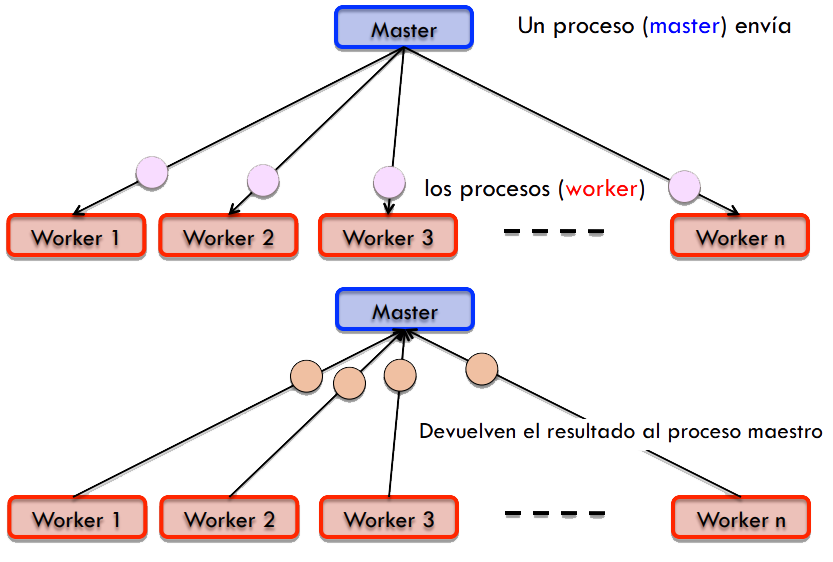
\includegraphics[width=0.65\textwidth]{images/chapter_2/mpi_1}
		\caption{Comunicación Master-Worker}
		\label{fig:comunicacion_mw}
	\end{figure}

	\newpage

	Esta técnica de paralelización utiliza memoria distribuida, es decir, cada proceso tiene su propia memoria local. Así, los procesos no tienen que preocuparse por los problemas de la memoria compartida, como la sincronización para el acceso de variables compartidas, condiciones de carrera o \textit{deadlocks} (dos o más procesos quedan bloqueados en un estado en el que ninguno puede continuar con su ejecución, pues están esperando a que otro proceso, también bloqueado, libere un recurso necesario para continuar). Asimismo, la memoria compartida no es fácilmente escalable a un gran número de procesadores\cite{jjruiz2016compartida}.


	Un programa ejecutado en paralelo, donde múltiples procesos se ejecutan en el mismo programa de manera independiente, pero trabajan con diferentes conjuntos de datos se denomina, por sus siglas en inglés, SPMD (Single Program Multiple Data). Este modelo es comúnmente utilizado en computación de alto rendimiento (HPC) y en entornos de procesamiento paralelo. La escalabilidad y eficiencia de este modelo son sus principales ventajas. Los mensajes pueden ser:
	\begin{itemize}
		\item Síncronos: El proceso receptor se queda bloqueado esperando el mensaje.
		\item Asíncrono: el receptor no se bloquea, por lo que puede adelantar código mientras espera a recibir el mensaje.		
	\end{itemize}

	
	Un programa MPI (ver Figura \ref{fig:ejecucion_mpi}), comparte el mismo código para todos los procesos ejecutados. Un proceso lee el conjunto de datos y los carga en su memoria, para luego dividirlos y enviarlos a los procesos disponibles. Una vez repartido el \textit{dataset}, se ejecutan en paralelo y procesan los datos recibidos. Cuando un proceso finaliza el procesado de los datos, envía los datos procesados al proceso correspondiente. La Figura \ref{fig:esquema_mpi} representa en código esta idea.
	
	\vspace{-0.2cm}
	
	\begin{figure}[!h]
		\centering
		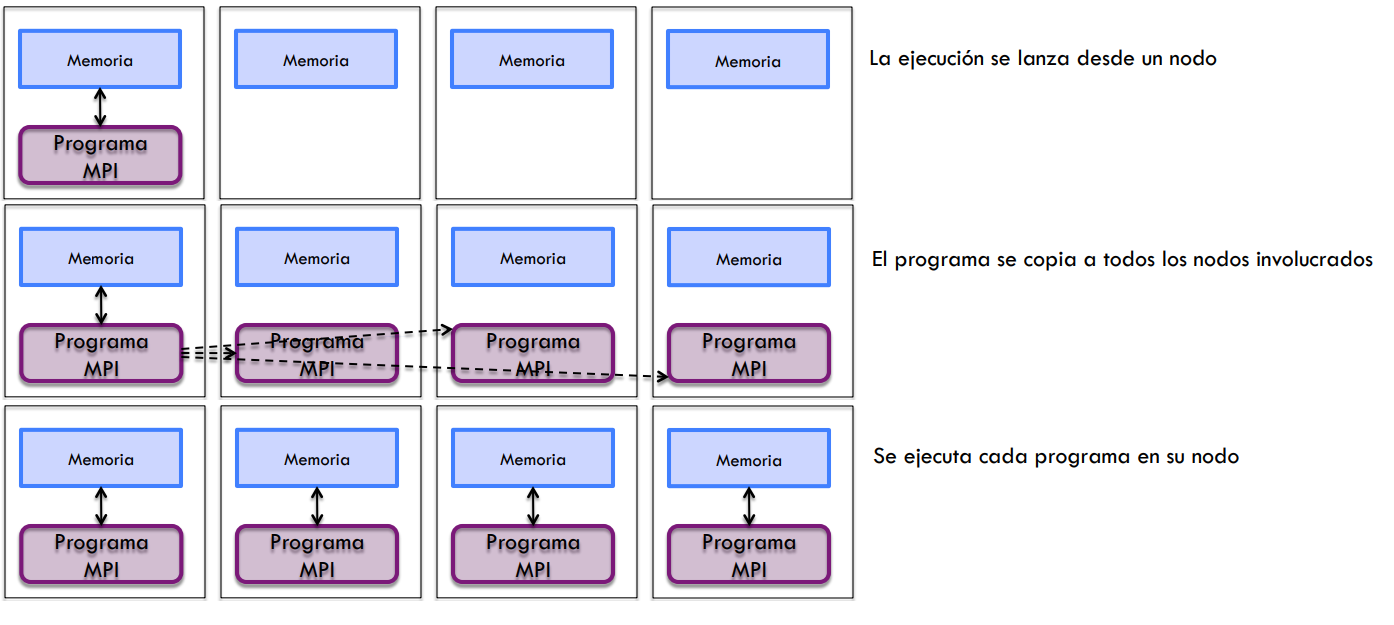
\includegraphics[width=0.90\textwidth]{images/chapter_2/mpi_2}
		\caption{Ejecución MPI}
		\label{fig:ejecucion_mpi}
	\end{figure}
	
	\vspace{-0.2cm}
	
	\vspace{-0.1cm}

	\begin{figure}[!h]
		\lstset{language=python, 
			language=python,
			breaklines=true,
			basicstyle=\footnotesize, %\footnotesize\ttfamily
			backgroundcolor=\color{lightergray},
			keywordstyle=\color{blue}, 
			commentstyle=\color{green!60!black},
			stringstyle=\color{purple}, 
			numbers=left, 
			numberstyle=\tiny\color{gray}, 
			frame=single,}
		
		\begin{lstlisting}[frame=single]
 from mpi4py import MPI # Al importar la biblioteca en Python se genera el entorno.

 comm = MPI.COMM_WORLD     	# Comunicador
 status = MPI.Status()   	# Status
 myrank = comm.Get_rank() 	# id de cada proceso
 numProc = comm.Get_size() 	# Numero de procesadores

 if myrank==0:           	# Master
    # Carga el conjunto de datos. Los divide y envia.
    # Recibe todos los datos procesados.
 else:                   	# Workers
    # Recibe el subconjunto de datos que le asigna el Master.
    # Procesa los datos. Los envia.
		\end{lstlisting}
		\caption{Esquema básico para ejecutar un programa MPI en Python}
		\label{fig:esquema_mpi}
	\end{figure}
	
	\newpage

\section{Aprendizaje por Refuerzo}
\label{cap:2_2}
	Reinforcement Learning (RL, por sus siglas en inglés), en español, Aprendizaje por Refuerzo, es un tipo de aprendizaje automático donde el agente aprende en base a las decisiones tomadas al interactuar con el entorno. El agente aprende a cumplir un objetivo en un entorno ejecutando un determinado número de acciones. Este tipo de algoritmos no requiere de entradas etiquetadas como en el aprendizaje supervisado, sino que recibe una retroalimentación, \textit{feedback} en inglés (recompensas o castigos), al realizar acciones en los estados. Aprendiendo con prueba y error, el agente explora el entorno para almacenar las mejores acciones para cada estado. 

	\begin{flushleft}
		Los componentes esenciales del algoritmo son los siguientes:
	\end{flushleft}
	\begin{itemize}
		\item \textit{Agente} que interactúa con el entorno y aprende de él, ejecutando sus acciones. 
		\item \textit{Entorno} con el cual el agente interactúa. Responde a las acciones tomadas por el agente y provee el \textit{feedback}.
		\item Conjunto de acciones o \textit{decisiones} que el agente puede realizar.
		\item \textit{Estados}, son las configuraciones que el entorno puede tomar.
		\item \textit{Feedback}, recompensas o castigos del entorno al realizar una acción en un estado.		
		\item Condición de \textit{finalización}. La cual puede ser desde encontrar la función óptima, hasta realizar un número de acciones.
	\end{itemize}


	\subsection{Algoritmo Q-Learning} 
		El algoritmo Q-Learning es una mezcla entre programación dinámica y Monte Carlo \cite{wang2012monte}. Es el más básico de entre los algoritmos de aprendizaje por refuerzo. Se usa para encontrar la mejor política de selección de acciones para un proceso de Decisión de Markov Determinado (MDP, por sus siglas en inglés) \cite{garcia2013markov}. 
		
		El procedimiento se realiza actualizando iterativamente las estimaciones de calidad de realizar dicha acción en el estado actual, conocido como valor-Q. Se suele representar en forma de matriz \textit{Q(S,A)}, guardando los valores-Q de las acciones en los estados. Este valor representa cómo de buena es la acción a realizar en un estado después de realizar una etapa de entrenamiento. Para ello, la Figura \ref{fig:qvalue} muestra la fórmula para actualizar los valores, para cada acción tomada por el agente.
				
		
		\begin{figure}[!h]				
		\begin{flushleft}
		\begin{mdframed}[roundcorner=5pt]
			\[
			Q(S,A) = (1 - \alpha) Q(S,A) + \alpha \left( R(S,A) + max_{i} \{ Q(S',A_i) \} \right)
			\]
			\begin{itemize}
				\item \( Q(S,A) \) ← Es el valor-Q de ejecutar la acción \( A \) en el estado \( S \).
				\item \( R(S,A) \) ← Es la recompensa obtenida al ejecutar la acción \( A \) en el estado \( S \).
				\item \( \alpha \) ← Tasa de aprendizaje. Controla cuánta importancia le da a la nueva información frente a la antigua.
				\item \( \gamma \) ← Factor de descuento. Determina la importancia de futuras recompensas comparadas con las recompensas inmediatas.
				\item \( max_{i}(Q(S',A_i)) \) : Es el valor máximo obtenible de realizar las posibles acciones en el estado siguiente.
			\end{itemize}
		\end{mdframed}		
		\end{flushleft}
		\caption{Cálculo del Q-Value de un estado y acción}	
		\label{fig:qvalue}
		\end{figure}
		
		
		El agente toma la decisión de ejecutar una acción dependiendo del hiper-parámetro $\epsilon$  con valores entre \textit{[0,1]}. Con un número aleatorio (en el mismo intervalo) calcula la probabilidad de ejecutar la mejor acción aprendida hasta el momento, o una acción aleatoria entre las disponibles. Si el valor es alto, con alta probabilidad se ejecutará la mejor acción aprendida hasta el momento, y es posible que no aprenda otras formas de alcanzar el objetivo.
		
		%\newpage
		
		Este algoritmo se ha aplicado en muchos dominios, como puede ser videojuegos de Atari \cite{mnih2013playing}, robótica o problemas de optimización. Sin embargo, sufre cuando el entorno tiene muchos estados, ya que la complejidad espacial aumenta considerablemente, y no resulta práctico contar con dos matrices. Por eso se diseñó el algoritmo DQN, el cual usa una red neuronal. Así, se elimina la maldición de dimensionalidad \cite{kuo2005lifting}, problemas que surgen con el exceso de variables independientes en un \textit{dataset}. En este algoritmo, el problema es el elevado número de estados que el agente ha de recorrer.
		
	\subsection{Deep Q-Network (DQN)}
	\label{cap:2_2_2}
		Debido a los problemas de escalabilidad mencionados anteriormente, se desarrolló el algoritmo de Redes Neuronales Profundas (DQN, por sus siglas en inglés). Este algoritmo combina redes neuronales con la base de aprendizaje por refuerzo, eliminando así la Q-Table.
		
		La estructura de la red neuronal depende del entorno del problema. Los valores de la capa oculta se pueden modificar dependiendo de las necesidades del programador, pero la capa de entrada y salida depende del problema. La entrada se adapta para recibir un estado del entorno, como por ejemplo una imagen representada como una matriz. La salida de la red tendrá tantos nodos como acciones tenga el agente. 
		
		En este trabajo, el entorno del problema será el juego Pacman, diseñado por la empresa \textit{Namco}, y en particular la versión de \textit{Atari 2600}, (ver Figura \ref{fig:pacman}). El juego consiste en recolectar todas las monedas del laberinto sin ser comido por un fantasma. Implementamos el juego -desde cero- para moldear según nuestros intereses la implementación y que el algoritmo DQN sea más eficiente y sencillo. En el Capítulo \ref{cap:c3_implementaciones}, diseño e implementaciones, se desarrolla en profundidad.
		
		\begin{figure}[!h]			
			\centering
			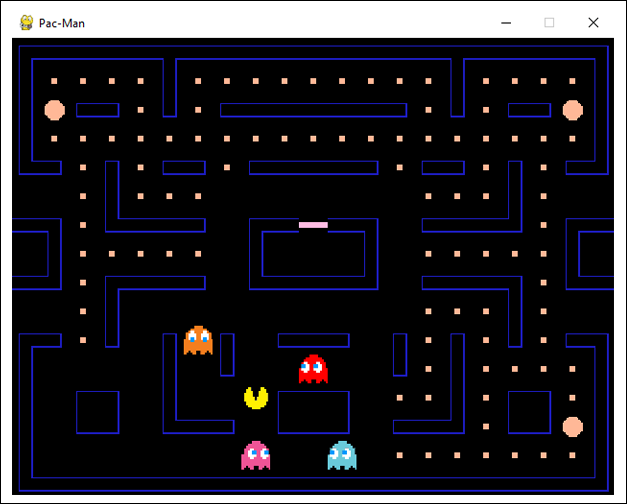
\includegraphics[width=0.55\textwidth]{images/chapter_2/pacman}	
			\caption{Juego Pac-Man implementado desde cero. Versión Atari 2600}
			\label{fig:pacman}
		\end{figure}
		
		
		
		El algoritmo DQN a realizar tendrá dos redes neuronales, una del estado actual y otra de anticipo, es decir, el siguiente estado. Esto sirve para ayudar a tener más contexto del estado actual, pues con una sola imagen (estado del juego), la información del estado puede variar considerablemente. En la fase de entrenamiento se realizan varios episodios, que consisten en ejecuciones hasta que se dé una condición de finalización. Además de ejecutar repeticiones de estados guardados anteriormente (replay buffer). En este algoritmo se usan tres hiper-parámetros: 
		\begin{enumerate}
			\item \textit{Gamma}, factor de descuento [0, 1]. Utilizado para saber cuánto resta a la recompensa adquirida al realizar una acción en un estado.
			\item \textit{Epsilon}, tasa de exploración [0, 1]. Probabilidad utilizada para ejecutar una acción aleatoria o la mejor hasta el momento. 
			\item \textit{Learning rate}, tasa de aprendizaje [0, 1]. Para la propagación hacia atrás de las redes neuronales. Esencialmente, mide cuánto cambian los pesos de los nodos al tener un fallo.
		\end{enumerate}	
		
		Además de estos parámetros, el algoritmo cuenta con otras variables para desarrollar las redes neuronales. 
		\begin{itemize}
			\item \textit{Epsilon decay}. Utilizado para no usar siempre el mismo valor de \textit{epsilon}. Esta variable marca cuanto se reduce la variable \textit{epsilon} entre episodios.
			\item Número de ejemplos de entrenamiento (\textit{batch size)}. Se utiliza para actualizar los parámetros de la red neuronal durante una sola iteración del entrenamiento.
			\item Tamaño de la capa oculta. Marca el número de neuronas en cada capa.
		\end{itemize}
		
		
		
		
		
	

\section{Aprendizaje No-Supervisado}

	Los métodos no supervisados (unsupervised methods, en inglés) son algoritmos de aprendizaje automático que basan su proceso en un entrenamiento con datos sin etiquetar. Es decir, a priori, no se conoce ningún valor objetivo, ya sea categórico o numérico. La meta de este aprendizaje es encontrar patrones o estructuras en los datos proporcionados. Estos algoritmos son útiles en escenarios en los cuales hay escasez de datos etiquetados o éstos no están disponibles.
	
	Hay muchos tipos de técnicas de aprendizaje no supervisado como, entre otros, la detección de anomalías, reducción de dimensionalidad o \textit{clustering}. En este proyecto vamos a reducir el tiempo de ejecución de las técnicas de \textit{clustering} que se encargan de agrupar individuos basándose en alguna medida de similitud. Como no es aprendizaje supervisado, no disponemos de información categorizada previamente, por lo que hay que calcular el número óptimo de \textit{clusters}. Para ello, hay medidas ya estudiadas como el diagrama de ``codo'', cuyo valor óptimo de \textit{clusters} se calcula visualmente, cuando empieza a crearse un codo (la diferencia con el número anterior no es tan pronunciada como en puntos anteriores). Hay otros coeficientes que calculan la optimalidad con algoritmos, como el coeficiente de Davies-Bouldin, cuyo valor mínimo indica el número óptimo de \textit{clusters}, o el coeficiente de Silhouette, similar al anterior, pero con el valor máximo. Se pueden apreciar los diferentes coeficientes para una misma categorización en la Figura \ref{fig:coeficientes}. Como se puede apreciar, el diagrama de codo es el coeficiente más complicado de visualizar, lo otros dos coeficientes solo es necesario encontrar el menor o mayor valor, mientras que en el primero hay que visualizar el codo, y en este ejemplo se podría elegir también tres \textit{clusters} como número óptimo.


	\begin{figure}[!h]
		\centering
		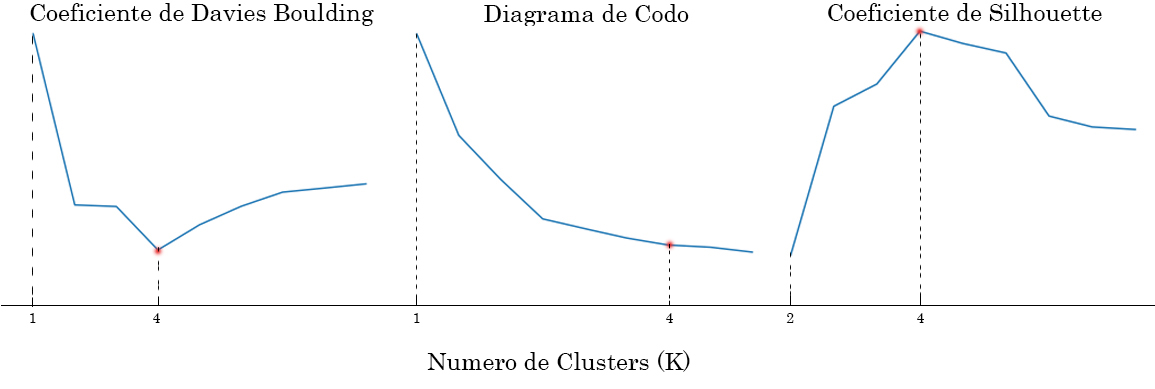
\includegraphics[width=0.95\textwidth]{images/chapter_2/ap_nosup_diagramas}
		\caption{Coeficientes de agrupación}
		\label{fig:coeficientes}
	\end{figure}
	


	Los llamados métodos jerárquicos \cite{ackermann2014analysis} tienen por objetivo agrupar \textit{clusters} para formar uno nuevo o bien separar alguno ya existente para dar origen a otros dos, de tal forma que, si sucesivamente se va efectuando este proceso de aglomeración, se minimice alguna distancia o bien se maximice alguna medida de similitud.
	
	\newpage

	\subsection{Clustering jerárquico aglomerativo}

		Este algoritmo usa una matriz para realizar la agrupación de los individuos. Comienza teniendo N \textit{clusters}, uno por cada individuo de la población. La matriz se representa por las filas, es decir, la fila i-ésima representa el \textit{cluster} i-ésimo. La matriz se rellena con las distancias entre los \textit{clusters}, por lo que la celda \textit{(i, j}) representa la distancia entre el \textit{cluster} \textit{i} y el \textit{j}.  
		
		En cada iteración, se busca en la matriz la celda \textit{(i, j)} con menor valor (distancia mínima), y se juntan los \textit{clusters} que representan la fila \textit{i} con la columna \textit{j}. La matriz se actualiza, eliminando la fila y la columna con mayor índice (entre \textit{i}, \textit{j}), y actualizando la fila y columna de menor índice. Este proceso se repite hasta que solo haya un \textit{cluster}. Las distancias entre \textit{clusters} pueden ser:
		\begin{itemize}
		\vspace{-0.25cm}
		\item Centroides: cada \textit{cluster} tiene un centro.
		\vspace{-0.25cm}
		\item Enlace simple o compuesto: la distancia entre \textit{clusters} viene dada por la menor o mayor distancia, respectivamente, entre los individuos que representan cada \textit{cluster}.
		\vspace{-0.30cm}
		\end{itemize}



		\begin{algorithm}[!h]
			\caption{Jerárquico Aglomerativo}
			\KwData{poblacion, C  // Numero de clusters deseados}
			\KwResult{agrupacion // Clusters para cada individuo de la poblacion}
			D := init() // Inicializar la matriz de distancias\\
			\While{number of rows in $matrix$ $> C$}{
				// Recorre la matriz en búsqueda del menor valor (i, j)\\
				i, j :=busqueda\_min(poblacion)\\
				// Agrupa los cluster (i, j)\\
				agrupacion := agrupar\_clusters(poblacion, i, j)\\
				// Elimina la fila y columna de mayor índice\\
				eliminar\_cluster(poblacion, max(i, j))\\	
				// Calcula nuevas distancias al cluster agrupado (i)
				nuevas\_distancias(poblacion, min(i, j))
			}
			
		\end{algorithm}
		\vspace{-0.20cm}

		La complejidad en los enlaces simple y completo tienen un coste cúbico O(\(N^{3}\)), al tener que comparar todos los individuos uno a uno entre dos \textit{clusters}.
		

		Al finalizar la ejecución se puede representar la agrupación mediante un dendograma \cite{espinoza2012using} (ver Figura \ref{fig:dendograma}), y comprobar el número óptimo de \textit{clusters} para la población calculada. Sin embargo, no es igual de preciso que los coeficientes mencionados anteriormente. 
		
		\begin{figure}[!h]
			\centering
			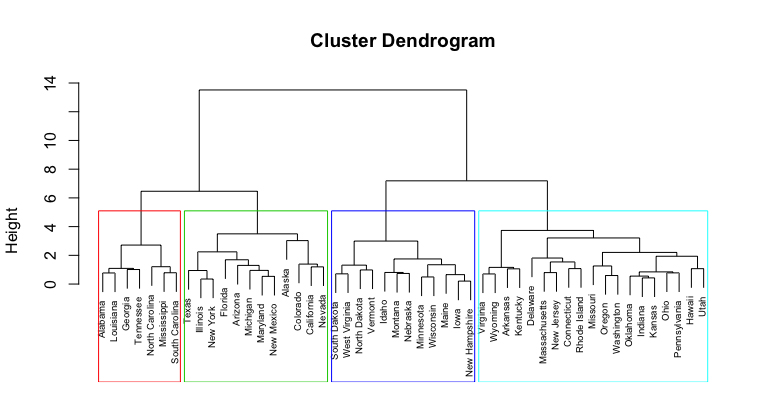
\includegraphics[width=0.75\textwidth]{images/chapter_2/dendograma}
			\caption{Dendograma de una población de 20 individuos}
			\label{fig:dendograma}
		\end{figure}


	\subsection{Clustering basado en particiones: K-Medias}

		La meta de este algoritmo es particionar la población inicial en \textit{K} \textit{clusters}, donde cada individuo se agrupa con el \textit{cluster} más próximo. El algoritmo itera en un bucle en el cual calcula la asignación de todos los individuos. Al final de cada iteración calcula los nuevos centros, si estos no cambian con respecto a la iteración anterior, termina la ejecución. La optimalidad de la agrupación se calcula mediante el sumatorio de las distancias de todos los individuos y los centroides de sus \textit{clusters}. 
		
		
		\begin{algorithm}[!h]
			\caption{K-Medias}
			\KwData{poblacion, K}
			\KwResult{agrupacion}
			centrosNuevos := init(K) // Inicializa los centros de manera aleatoria\\
			
			\Repeat{$centros$ $!= centrosNuevos$}
			{
				centros := centrosNuevos\\
				// Asigna a cada individuo el cluster mas cercano\\
				agrupacion := asignar(poblacion, centros)\\
				// Calcula las posiciones de los nuevos centros\\
				centrosNuevos := calculaCentros(poblacion, asignacion)
			}
			
			
			\Return $agrupacion$\;
		\end{algorithm}
		
		Sin embargo, hay que tener en cuenta que la inicialización de los centros es estocástica, por lo que el algoritmo puede converger en un óptimo local. Por eso es importante repetir el algoritmo varias veces para encontrar el óptimo general. La Figura \ref{fig:kmediasBusqueda} muestra un ejemplo de ejecución, junto con la búsqueda de la mejor agrupación. Esta figura representa la búsqueda al ejecutar tres veces el algoritmo. El intento con menor valor del sumatorio de distancias de individuos, y su \textit{cluster} asignado, es la mejor asignación entre los intentos ejecutados. El tercer intento es la agrupación que muestra la figura.


		\begin{figure}[!h]
			\centering
			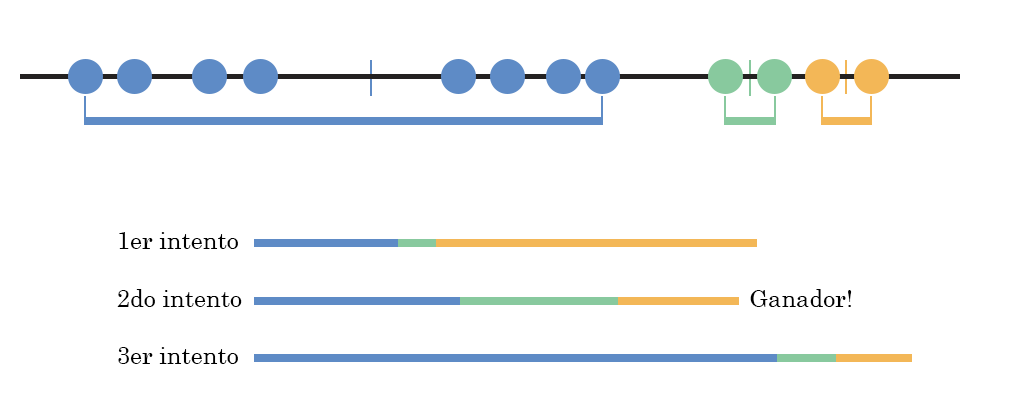
\includegraphics[width=1\textwidth]{images/chapter_2/kmedias}
			\caption{Búsqueda del óptimo general en el algoritmo de K-Medias}
			\label{fig:kmediasBusqueda}
		\end{figure}


\section{Aprendizaje Supervisado}
	Al contrario que el apartado anterior, este tipo de aprendizaje automático es entrenado con un \textit{dataset} categorizado con su salida correcta. El algoritmo aprende de este conjunto para hacer predicciones sobre unos datos desconocidos.
	
	El objetivo de este algoritmo es aprender la función que mapea las variables de entrada en las categorías correctas de salida. Para ello, ajusta los parámetros con técnicas de optimización iterativas para minimizar el error en sus predicciones.
	
	Los ejemplos más comunes son la clasificación, para dividir la población en categorías según unos parámetros, y regresión, que encuentra las correlaciones entre las variables dependientes e independientes.


	\subsection{K-Vecinos más Cercanos - KNN}

		KNN (K-Nearest Neighbors en inglés) es un algoritmo simple pero potente, resultando muy efectivo para tareas de clasificación y regresión. Se basa en la idea de que los puntos de datos similares tienden a agruparse en el espacio de características. Este algoritmo pertenece al paradigma de aprendizaje perezoso o basado en instancias.
		
		\begin{itemize}
			\item Perezoso: no calcula ningún modelo y demora todos los cálculos hasta el momento en que se le presenta un ejemplo nuevo.			
			\item Basado en instancias: usa todos los individuos disponibles y ante un ejemplo nuevo recupera los más relevantes para componer la solución.	
		\end{itemize}
		
		No hay una forma de determinar el mejor valor para K, de forma que hay que probar con varias ejecuciones. Valores pequeños de K crea sonido, provocando que inicialmente se categorice con un \textit{cluster} no idóneo, y a la larga se categoricen muchos de forma incorrecta. Valores grandes con pocos datos favorece a los \textit{clusters} con más individuos. Un valor diferente de K puede cambiar la categoría de un individuo. En la imagen izquierda de la Figura \ref{fig:aprendizaje_supervisado} se puede apreciar el proceso de asignación de un \textit{cluster} a un nuevo individuo. Como se puede ver con los círculos que delimitan los K vecinos más cercanos, si variamos K, la asignación del nuevo individuo puede cambiar.

		\begin{algorithm}
			\caption{K-Vecinos más Cercanos}
			\KwData{poblacion, etiquetas, poblacionPred, K}
			\KwResult{agrupacion // Clusters para cada individuo de la población}
			agrupacion := $\emptyset$\\
			\For{each individuo $ind$ in $poblacionPred$}{
				// Recorre toda la población guardando los K individuos más cercanos\\
				vecinos := recorrer\_poblacion(poblacion, individuo, K)\\
				// Clasifica según los K vecinos\\
				cluster := clasificar\_individuo(vecinos)\\
				agrupacion.append(cluster)
			}
			\Return $agrupacion$
		\end{algorithm}
		
		La distancia entre individuos más usada es la Euclídea, pero requiere más tiempo al aplicar potencias y raíces cuadradas en su cálculo. La distancia Manhattan es más rápida, pero menos precisa.



		%\begin{figure}[!h]
		%	\centering
		%	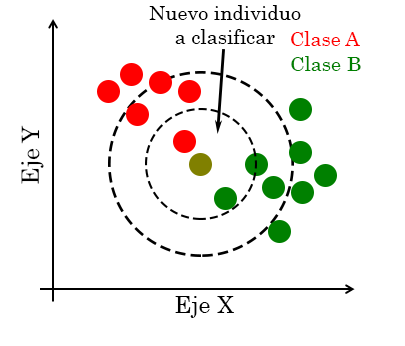
\includegraphics[width=0.5\textwidth]{images/chapter_2/knn}
		%	\caption{KNN}
		%	\label{fig:knn}
		%\end{figure}
		
		
		\begin{figure}[!ht]
			\centering
			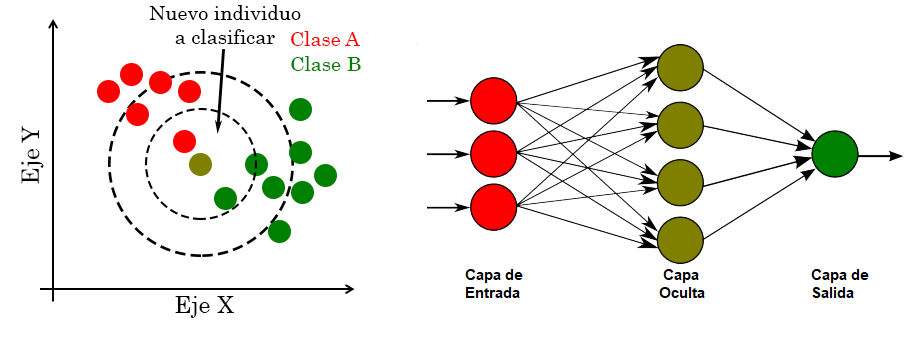
\includegraphics[width=\textwidth]{images/chapter_2/knn_redneu}
			\caption{Algoritmos de aprendizaje supervisado}
			\label{fig:aprendizaje_supervisado}
		\end{figure}

	\subsection{Redes Neuronales}

		Las redes neuronales son un modelo computacional inspirado en el funcionamiento y estructura de las neuronas del cerebro humano. Esencialmente, consisten en capas de nodos interconectados, llamadas neuronas artificiales. La estructura del modelo se muestra en la imagen de la derecha de la Figura \ref{fig:aprendizaje_supervisado}. En este modelo se aprecian:


		\begin{itemize}
			\item Capa de entrada, en la cual, habrá tantas neuronas como variables de entrada tenga el modelo de predicción.
			\vspace{-0.4cm} 
			\item Capa oculta, representada con una o más capas internas. Cada una contiene un número determinado de neuronas.
			\vspace{-0.4cm}	
			\item Capa de salida. Como en la entrada, tendrá un número de neuronas relacionadas con las variables de salida.
		\end{itemize}
		
		\vspace{-0.2cm}
		
		Se ha demostrado que las redes neuronales tienen un rendimiento notable en muchas tareas, como el reconocimiento de imágenes o procesamiento de lenguaje natural. Aprenden patrones complejos al someterse a un entrenamiento específico con un amplio \textit{dataset} categorizado.	
		
		%\begin{figure}[!h]
		%	\centering
		%	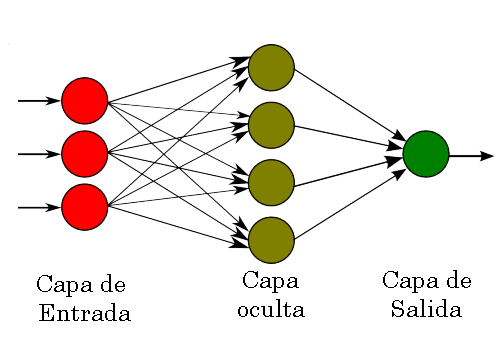
\includegraphics[width=0.5\textwidth]{images/chapter_2/redneu}
		%	\caption{Red Neuronal}
		%	\label{}
		%\end{figure}
		
		En el proceso de entrenamiento aprende a realizar una tarea específica ajustando los parámetros internos (pesos en las conexiones), gracias al \textit{dataset} proporcionado. Normalmente, este ajuste se lleva a cabo con algoritmos de optimización como descenso de gradiente, donde se comparan las predicciones del modelo con la categoría correcta, y se actualizan los parámetros del modelo con un método de propagación hacia atrás, \textit{backpropagation} en inglés. Estos valores se actualizan dependiendo del error cometido y la tasa de aprendizaje proporcionada al modelo.
		
		El Algoritmo \ref{alg:redneu} muestra la etapa de entrenamiento a la cual una red neuronal se somete para poder cambiar los pesos de las neuronas y poder obtener un funcionamiento correcto con respecto a los valores entrenados.



		\begin{algorithm}
			\caption{Red Neuronal}
			\label{alg:redneu}
			\KwData{entrenamiento, etiquetas, evaluacion // Individuos sin categorizar\\
					\Indp \Indp repeticiones, capas // Tam. entrada, oculta, salida}
			\KwResult{pesos // Opcionalmente, devolver los pesos de la red}
			pesos := init() // Inicializar los pesos de manera aleatoria\\
			\For{$rep \leftarrow 0$ \KwTo $repeticiones$}{
				cont := 0\\
				\For{each $ind$ in $entrenamiento$}{
					// Suma el valor recibido de la capa anterior multiplicada por los pesos de la capa actual con la siguiente. Así se determina la importancia de conexión entre las neuronas. Con el valor calculado se aplica a una función de activación y se pasa a la siguiente capa hasta llegar a la salida.\\			
					predicion := \textbf{forward(pesos, ind)}\\
					// El valor predicho calculado en la salida es comparado con la etiqueta, y se calcula el error. Este error se manda para atrás actualizando los pesos. Se suma la multiplicación del valor predicho en cada capa con la tasa de aprendizaje y el error.\\			
					\textbf{backpropagation(pesos, predicion, etiqueta[cont])}
					cont++
				}
			}
			
			
			\Return $agrupacion$
		\end{algorithm}



		%\vspace{0.2cm}
		
		%\begin{figure}[!h]
		%	\centering
		%	
		%	
		%	\begin{subfigure}[t]{0.33\textwidth}
		%		\centering
		%		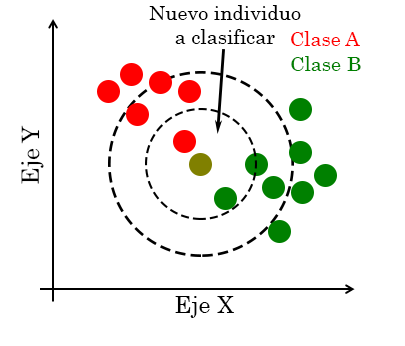
\includegraphics[width=\textwidth]{images/chapter_2/knn}
		%		\caption{KNN}
		%		\label{fig:knn}
		%	\end{subfigure}
		%	\hfill
		%	\begin{subfigure}[t]{0.48\textwidth}
		%		\centering
		%		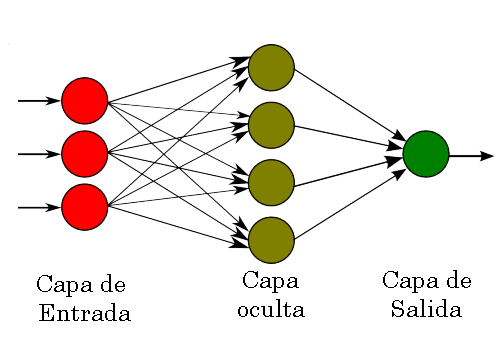
\includegraphics[width=\textwidth]{images/chapter_2/redneu}
		%		\caption{Red Neuronal}
		%		\label{fig:redneu}
		%	\end{subfigure}
		%	
		%	\caption{Aprendizaje Supervisado}
		%	\label{fig:aprendizajeSupervisado}
		%\end{figure}
		









\section{Algoritmos Evolutivos}


	La programación evolutiva es una técnica de optimización inspirada en la teoría de la evolución biológica. Se basa en el concepto de selección natural y evolución de las poblaciones para encontrar soluciones a problemas complejos. 
	
	La población está compuesta por individuos, que pueden ser representados con arrays de números reales, binarios o un árbol, en programación genética. Los individuos tienen un cromosoma, que a su vez tiene uno o varios genes, con uno o más alelos. Esta población es sometida a métodos de evaluación, selección, cruce y mutación para, con el paso de las generaciones, maximizar o minimizar un valor \textit{fitness}.
	
	Esta técnica es muy útil para problemas de optimización donde los métodos tradicionales no proporcionan el rendimiento deseado. Los Algoritmos Evolutivos se han aplicado a varios dominios, como por ejemplo la bioinformática o robótica \cite{contreras2015mobile}.
	
	La Figura \ref{fig:AG} muestra el diagrama de estados del algoritmo más básico. Cada método se puede modificar para cualquier individuo, así como añadir más técnicas para garantizar y/o mejorar los resultados finales, como puede ser el elitismo, que garantiza la supervivencia de los mejores individuos, o un desplazamiento de los valores \textit{fitness} para evitar valores negativos. 


	\begin{figure}[!h]
		\centering
		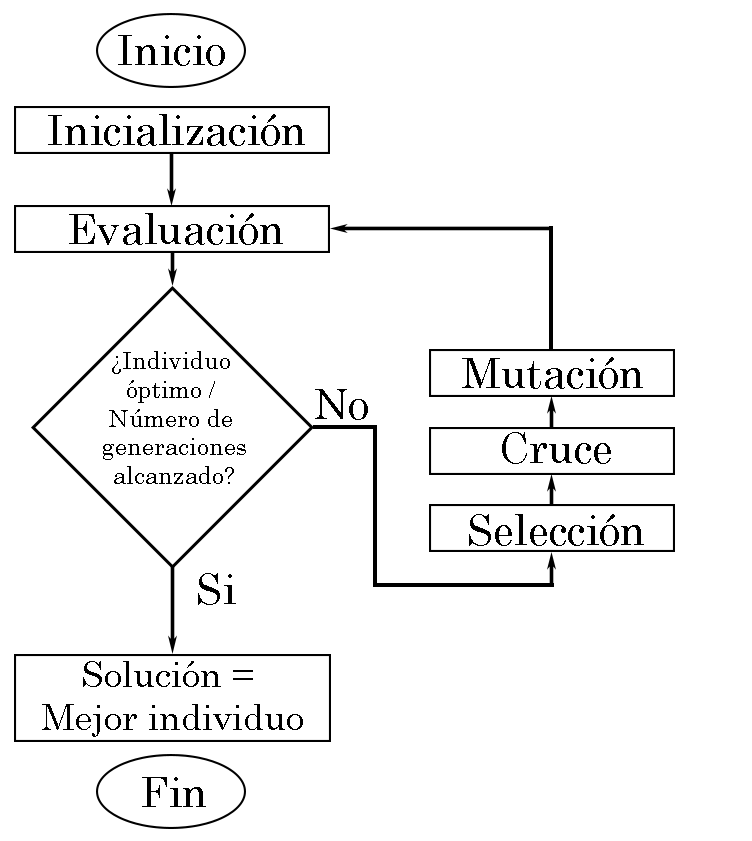
\includegraphics[width=0.50\textwidth]{images/chapter_2/AG}
		\caption{Algoritmo Evolutivo básico}
		\label{fig:AG}
	\end{figure}




%Aquí comienza la descripción del trabajo realizado. Se deben incluir tantos capítulos como sea necesario para describir de la manera más completa posible el trabajo que se ha llevado a cabo. Como muestra la figura \ref{fig:sampleImage}, está todo por hacer.
%
%\begin{figure}[h]
%	\centering
%	\includegraphics[width = 0.5\textwidth]{Imagenes/Vectorial/Todo.pdf}
%	\caption{Ejemplo de imagen}
%	\label{fig:sampleImage}
%\end{figure}
%
%Si te sirve de utilidad,  puedes incluir tablas para mostrar resultados, tal como se ve en la tabla \ref{tab:sampleTable}.
%
%
%\begin{table}
%	\centering
%	\begin{tabular}{c|c|c}
%		\textbf{Col 1} & \textbf{Col 2} & \textbf{Col 3} \\
%		\hline\hline
%		3 & 3.01 & 3.50\\
%		6 & 2.12 & 4.40\\
%		1 & 3.79 & 5.00\\
%		2 & 4.88 & 5.30\\
%		4 & 3.50 & 2.90\\
%		5 & 7.40 & 4.70\\
%		\hline
%	\end{tabular}
%	\caption{Tabla de ejemplo}
%	\label{tab:sampleTable}
%\end{table}

\include{Capitulos/3_Diseño_implementaciones}
\include{Capitulos/4_Estudio_empírico}
\chapter{Conclusiones y trabajo futuro}
\label{cap:c5_conclu}

	En este trabajo se han desarrollado varias mejoras en distintos algoritmos de IA, a través de la biblioteca estándar de paso de mensajes MPI. Los desafíos encontrados durante su desarrollo resultaron ser más complejos de lo que se había previsto inicialmente. Los problemas de configuración de la biblioteca MPI en Windows, así como y adaptar la gestión de bibliotecas de Python usando Anaconda, fueron unos problemas completamente imprevistos. El desconocimiento general de  MPI se debe a la ausencia de asignaturas específicas de programación distribuidas en el grado de Ingeniería Informática, únicamente ofreciendo fundamentos teóricos, sin profundizar en la práctica. La ejecución de las pruebas en el sistema distribuido de la Facultad de Informática, junto con la documentación del trabajo desarrollado, tomó más tiempo del calculado. Sin embargo, fue una etapa sumamente gratificante e interesante. 
	
		
	Una vez finalizadas las estrategias propuestas, se ha llevado a cabo una fase de experimentación, que ha consistido en analizar los tiempos de ejecución, variando tanto los parámetros disponibles, como los conjuntos de poblaciones para cada tipo de algoritmo. Cabe destacar el alto coste computacional de los experimentos. Por ejemplo, en el algoritmo jerárquico aglomerativo con distancia por enlace simple, una prueba en el sistema  distribuido requirió más de un día en finalizar, obligando a reducir el tamaño de la población usada. Es importante remarcar que algunos de los resultados obtenidos no coincidían con la tendencia esperada. En particular, la estrategia de segmentación (pipeline) realizada en las redes neuronales, donde el rendimiento alcanzado fue peor que el algoritmo secuencial a pesar de contar con -al menos- tres procesos. Aparte de disponer con los resultados obtenidos en la misma estrategia, pero para los algoritmos evolutivos, en los cuales si se obtuvieron buenos resultados. Después de realizar un análisis, observamos que la causa de estos resultados se debe a contar con dos flujos de mensajes en direcciones opuestas. La importancia de los buenos resultados es equivalente a obtener resultados no tan eficaces como se esperaban, pues es un avance para extraer conclusiones u otras ideas a implementar.
	

	Una de las cosas más importantes que he aprendido a lo largo del trabajo es que no siempre \textit{más es mejor}. Utilizar más procesos no tiene por qué derivar en un rendimiento proporcional al trabajo ejecutado. La sobrecarga (\textit{overhead}) de los procesos en las implementaciones es un fundamento a tener en cuenta a la hora de ejecutar programas, y en la vida misma.	
	
	
	Como trabajo a futuro se propone investigar otros algoritmos de las técnicas desarrolladas, además de investigar y mejorar otras técnicas de IA, como puede ser el procesamiento del lenguaje natural.
	
	
	
	
	
%\input{chapter4.tex}
%\input{chapter5.tex}

% +-------------------------------------------------------------------------+
% | References                                                              |
% +-------------------------------------------------------------------------+

% +-------------------------------------------------------------------------+
% | In order for WinEDT to index references correctly, it has to know where |
% | the file resides.  The following command is prefaced by %, and will be  |
% | ignored completely by LaTeX.  However, WinEDT will use this line to     |
% | access the external .bib bibliography file.  Also note that WinEDT can  |
% | read file path names with either "\" or "/" - LaTeX, however, doesn't   |
% | like "\", so it's easier to store a path name in the "Unix" style.      |
% +-------------------------------------------------------------------------+

%Included for Gather Purpose only.  Do NOT uncomment:
%input "references.bib"

% +--------------------------------------------------------------------+
% | This template uses the BibTeX program to format references.  The
% | 3 lines below create a separate Bibliography section and add
% | an entry for "raphy" to the Table of Contents.  The actual
% | data for your references (author, title, journal, date, etc.) are
% | entered in the references.bib file.  See that file for information
% | on how to enter references.
% +--------------------------------------------------------------------+

\bibdata{references}
\bibliography{references}
\addcontentsline{toc}{chapter}{Bibliography}



% Fichero con acr�nimos para su uso con GlossTeX
%
% El listado de acr�nimos funciona de manera similar a las referencias
% bibliogr�ficas. Este  fichero es equivalente por tanto  al .bib, con
% el listado de  los acr�nimos disponibles. A lo  largo del documento,
% cuando se  utilice alguno  de ellos, se  referencia para  indicar al
% sistema que queremos que dicho  acr�nimo aparezca en el glosario. En
% contra de  lo que ocurre con  la bibliograf�a, el  texto original no
% sufre ninguna modificaci�n.
%
% Las entradas son:
% @entry{<etiqueta>[,<item>[,<forma larga>]]} [<texto>]
%
% La etiqueta es el  nombre del acr�nimo (equivalente a la etiqueta en
% BibTeX) que luego se utiliza para "referenciarlo" en el texto.

% Para  que  la  generaci�n   en  Release  con  el  Makefile  funcione
% correctamente, necesitar�s  al menos tener  referenciado un acr�nimo
% dentro del  texto.  Si  no quieres usar  acr�nimos, o de  momento no
% tienes ninguno  referenciado, basta con que no  definas la constante
% \acronimosEnRelease en config.tex





\begin{flushleft}
	\huge{\textbf{Acrónimos}}
\end{flushleft}

\vspace{1cm}

\textbf{MPAI} Message Passing Artificial Inteligence
\newacronym{MPAI}{MPAI}{Message Passing Artificial Inteligence}

\vspace{0.5cm}

\textbf{MPI} Message Passing Interface 
\newacronym{MPI}{MPI}{Message Passing Interface}

\vspace{0.5cm}

\color{blue} TODO... \color{black}




% +--------------------------------------------------------------------+
% | Finally, we generate the appendix.  To add or delete appendices,
% | add or remove the line
% |
% |     \input{appendixX.tex}
% |
% | where "X" is the letter designation of the Appendix (A, B, C, etc.)
% | You should have one \input{appendixX.tex} line and a corresponding
% | file appendixX.tex for each appendix.                                 |
% +--------------------------------------------------------------------+

%\appendix
%\input{appendixA.tex}
%\input{appendixB.tex}

\end{document}
